\section{Capítulo 3 -- Listas Encadeadas}

Em Algoritmos I você trabalhou com vetores: uma sequência de posições lado a lado na memória, com tamanho definido na criação. Neste capítulo você vai construir uma estrutura que cresce e encolhe conforme a necessidade, sem desperdiçar espaço e sem deslocar elementos: a \textbf{lista encadeada}. Ela é a primeira estrutura dinâmica do livro e a base de várias outras, como pilhas, filas e grafos.

\subsection{3.1 Quando o vetor não basta}

Imagine um sistema que registra os pedidos de uma loja ao longo do dia. Não dá para saber quantos pedidos vão chegar. Se você criar um vetor de 1.000 posições e chegarem 30 pedidos, desperdiçou memória; se chegarem 1.500, faltou espaço. O vetor dinâmico do Capítulo 1 resolve parte do problema, mas cada vez que enche precisa copiar tudo para um espaço maior.

Há um segundo problema: inserir ou remover \textbf{no meio}. Para colocar um pedido urgente na frente da fila de um vetor, todos os outros precisam andar uma posição. Com 1 milhão de pedidos, isso é 1 milhão de movimentações.

A lista encadeada resolve as duas questões com uma ideia simples: cada elemento fica em um \textbf{nó} criado separadamente na memória, e cada nó guarda, além do valor, um \textbf{ponteiro para o próximo}. Os nós podem estar em qualquer lugar da memória; o que os mantém em ordem são os ponteiros.

\begin{center}
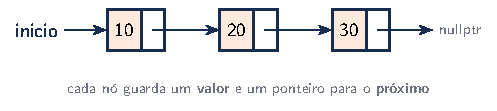
\includegraphics[width=0.9\linewidth,keepaspectratio]{imagens/capitulo-03_lista.pdf}
\end{center}

A lista só precisa guardar onde está o primeiro nó (\texttt{inicio}). A partir dele, seguindo os ponteiros, chega-se a todos os outros. O último nó aponta para \texttt{nullptr}, que marca o fim.

\subsection{3.2 Tipo Abstrato de Dados}

Antes de programar, vale separar duas perguntas: \textit{o que} a lista faz e \textit{como} ela faz. A resposta à primeira pergunta é a \textbf{interface}: o conjunto de operações que quem usa a lista pode chamar. Um \textbf{Tipo Abstrato de Dados} (TAD) é justamente isso: um tipo definido pelas operações que oferece, sem expor como elas são implementadas.

\begin{center}
\begin{tabular}{@{}p{0.34\linewidth}p{0.52\linewidth}@{}}
\toprule
\rowcolor{headergray}
\tblheader{Operação} & \tblheader{O que faz} \\
\midrule
\texttt{inserirInicio(v)} & coloca o valor \texttt{v} no começo \\
\rowcolor{rowgray} \texttt{inserirFim(v)} & coloca o valor \texttt{v} no final \\
\texttt{inserirNaPosicao(p, v)} & coloca \texttt{v} na posição \texttt{p} \\
\rowcolor{rowgray} \texttt{remover(v)} & retira a primeira ocorrência de \texttt{v} \\
\texttt{contem(v)} & diz se \texttt{v} está na lista \\
\rowcolor{rowgray} \texttt{quantidade()} & quantos elementos a lista tem \\
\texttt{vazia()} & diz se a lista está vazia \\
\bottomrule
\end{tabular}
\end{center}

A mesma interface poderia ser implementada com um vetor ou com nós encadeados. Quem usa a lista não precisa saber qual das duas foi escolhida: chama as mesmas operações e recebe os mesmos resultados. O que muda é o \textbf{custo} de cada operação, e é por isso que estudamos as implementações.

\subsection{3.3 O nó e a classe ListaEncadeada}

O nó é uma struct com o valor e o ponteiro para o próximo, como você viu no Capítulo 1. A lista é uma classe que guarda o ponteiro para o primeiro nó, um ponteiro para o último (veremos por quê) e a quantidade de elementos:

\begin{codigo}
\begin{Verbatim}[breaklines=true, breaksymbolleft={}, fontsize=\footnotesize]
// trecho: o nó e os dados da classe ListaEncadeada
struct No {
    int valor;
    No *proximo;
};

class ListaEncadeada {
private:
    No *inicio;    // primeiro nó (nullptr se a lista estiver vazia)
    No *fim;       // último nó
    int tamanho;   // quantidade de elementos
    // ... operações (a seguir)
};
\end{Verbatim}
\end{codigo}

Uma lista recém-criada não tem nós: \texttt{inicio} e \texttt{fim} valem \texttt{nullptr} e o tamanho é zero. Esse estado é a \textbf{lista vazia}, e toda operação precisa tratá-lo com cuidado.

\subsection{3.4 Inserindo elementos}

\subsubsection{No início: O(1)}

Inserir no início exige só dois passos, não importa quantos elementos a lista tenha: o novo nó aponta para o atual primeiro, e \texttt{inicio} passa a apontar para o novo nó.

\begin{center}
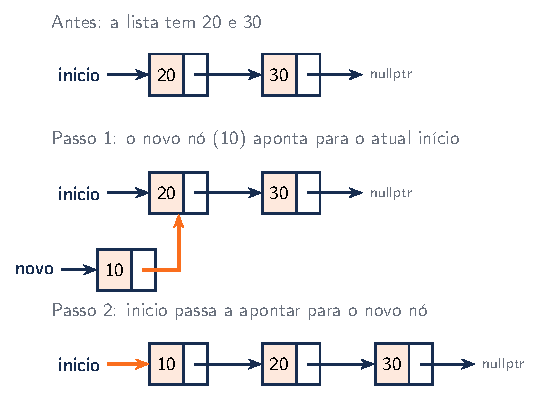
\includegraphics[width=0.95\linewidth,keepaspectratio]{imagens/capitulo-03_inserir_inicio.pdf}
\end{center}

\begin{codigo}
\begin{Verbatim}[breaklines=true, breaksymbolleft={}, fontsize=\footnotesize]
// trecho da classe ListaEncadeada
void inserirInicio(int valor) {
    No *novo = new No{valor, inicio};  // passo 1: aponta para o atual início
    inicio = novo;                     // passo 2: início passa a ser o novo nó
    if (fim == nullptr) {              // a lista estava vazia:
        fim = novo;                    // o novo nó também é o último
    }
    tamanho++;
}
\end{Verbatim}
\end{codigo}

A ordem dos passos importa. Se você fizer primeiro \texttt{inicio = novo}, perde a referência para o antigo primeiro nó, e o resto da lista fica inacessível.

\subsubsection{No fim: O(1) graças ao ponteiro fim}

Sem o ponteiro \texttt{fim}, inserir no final exigiria percorrer a lista inteira até achar o último nó: $O(n)$. Guardando um ponteiro para o último, basta ligá-lo ao novo nó:

\begin{codigo}
\begin{Verbatim}[breaklines=true, breaksymbolleft={}, fontsize=\footnotesize]
// trecho da classe ListaEncadeada
void inserirFim(int valor) {
    No *novo = new No{valor, nullptr};
    if (fim == nullptr) {        // lista vazia: o novo nó é o primeiro e o último
        inicio = novo;
        fim = novo;
    } else {
        fim->proximo = novo;     // o antigo último aponta para o novo
        fim = novo;              // e o novo passa a ser o último
    }
    tamanho++;
}
\end{Verbatim}
\end{codigo}

Esse é um exemplo de troca entre espaço e tempo: um ponteiro a mais na classe transforma uma operação $O(n)$ em $O(1)$.

\subsubsection{Em uma posição qualquer: O(n)}

Para inserir na posição \texttt{p}, é preciso caminhar até o nó da posição \texttt{p - 1} e ligar o novo nó depois dele. A caminhada custa $O(n)$; a ligação em si, $O(1)$.

\begin{codigo}
\begin{Verbatim}[breaklines=true, breaksymbolleft={}, fontsize=\footnotesize]
// trecho da classe ListaEncadeada
bool inserirNaPosicao(int pos, int valor) {
    if (pos < 0 || pos > tamanho) return false;          // posição inválida
    if (pos == 0) { inserirInicio(valor); return true; }
    if (pos == tamanho) { inserirFim(valor); return true; }

    No *anterior = inicio;
    for (int i = 0; i < pos - 1; i++) {                  // caminha até pos - 1
        anterior = anterior->proximo;
    }
    anterior->proximo = new No{valor, anterior->proximo};
    tamanho++;
    return true;
}
\end{Verbatim}
\end{codigo}

\subsection{3.5 Percorrendo e buscando}

Percorrer a lista é sempre o mesmo movimento: começar em \texttt{inicio} e seguir \texttt{proximo} até chegar em \texttt{nullptr}. Buscar um valor é percorrer comparando, e por isso custa $O(n)$ no pior caso, como a busca sequencial do Capítulo 2.

\begin{codigo}
\begin{Verbatim}[breaklines=true, breaksymbolleft={}, fontsize=\footnotesize]
// trecho da classe ListaEncadeada
bool contem(int valor) const {
    for (No *atual = inicio; atual != nullptr; atual = atual->proximo) {
        if (atual->valor == valor) {
            return true;
        }
    }
    return false;
}
\end{Verbatim}
\end{codigo}

Repare que não existe atalho para chegar ao quinto elemento: é preciso passar pelos quatro anteriores. Acessar uma posição por índice, que no vetor é $O(1)$, na lista encadeada é $O(n)$. Essa é a principal desvantagem da lista.

\subsection{3.6 Removendo elementos}

Para remover um nó, o nó \textbf{anterior} a ele passa a apontar para o \textbf{seguinte}. O nó removido fica fora da corrente e pode ser liberado com \texttt{delete}.

\begin{center}
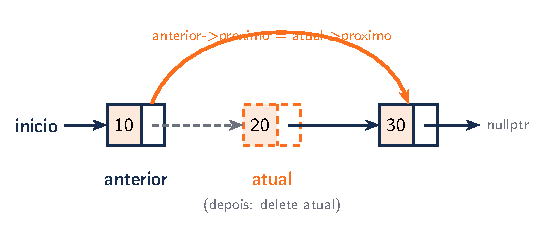
\includegraphics[width=0.9\linewidth,keepaspectratio]{imagens/capitulo-03_remover.pdf}
\end{center}

Como cada nó só conhece o próximo, a busca precisa andar com \textbf{dois ponteiros}: \texttt{atual}, que procura o valor, e \texttt{anterior}, que fica um passo atrás. A remoção ainda precisa tratar casos especiais: lista vazia, valor ausente, remoção do primeiro nó e remoção do último.

\begin{codigo}
\begin{Verbatim}[breaklines=true, breaksymbolleft={}, fontsize=\footnotesize]
// trecho da classe ListaEncadeada
bool remover(int valor) {
    No *anterior = nullptr;
    No *atual = inicio;
    while (atual != nullptr && atual->valor != valor) {
        anterior = atual;
        atual = atual->proximo;
    }
    if (atual == nullptr) {              // não encontrou (ou lista vazia)
        return false;
    }
    if (anterior == nullptr) {           // era o primeiro nó
        inicio = atual->proximo;
    } else {                             // estava no meio ou no fim
        anterior->proximo = atual->proximo;
    }
    if (atual == fim) {                  // era o último nó
        fim = anterior;
    }
    delete atual;
    tamanho--;
    return true;
}
\end{Verbatim}
\end{codigo}

\subsection{3.7 O programa completo}

Juntando as operações, a classe fica assim. Repare no destrutor, que percorre a lista liberando cada nó, e nas duas linhas com \texttt{= delete}, explicadas logo depois do código.

\begin{codigo}
\begin{Verbatim}[breaklines=true, breaksymbolleft={}, fontsize=\footnotesize]
struct No {
    int valor;
    No *proximo;
};

class ListaEncadeada {
private:
    No *inicio;
    No *fim;
    int tamanho;

public:
    ListaEncadeada() : inicio(nullptr), fim(nullptr), tamanho(0) {}

    // libera todos os nós quando a lista deixa de existir
    ~ListaEncadeada() {
        No *atual = inicio;
        while (atual != nullptr) {
            No *seguinte = atual->proximo;  // guarda antes de apagar
            delete atual;
            atual = seguinte;
        }
    }

    // impede cópias: duas listas não podem dividir os mesmos nós
    ListaEncadeada(const ListaEncadeada &) = delete;
    ListaEncadeada &operator=(const ListaEncadeada &) = delete;

    bool vazia() const { return tamanho == 0; }
    int quantidade() const { return tamanho; }

    void inserirInicio(int valor) {
        No *novo = new No{valor, inicio};
        inicio = novo;
        if (fim == nullptr) {
            fim = novo;
        }
        tamanho++;
    }

    void inserirFim(int valor) {
        No *novo = new No{valor, nullptr};
        if (fim == nullptr) {
            inicio = novo;
            fim = novo;
        } else {
            fim->proximo = novo;
            fim = novo;
        }
        tamanho++;
    }

    bool inserirNaPosicao(int pos, int valor) {
        if (pos < 0 || pos > tamanho) return false;
        if (pos == 0) { inserirInicio(valor); return true; }
        if (pos == tamanho) { inserirFim(valor); return true; }
        No *anterior = inicio;
        for (int i = 0; i < pos - 1; i++) {
            anterior = anterior->proximo;
        }
        anterior->proximo = new No{valor, anterior->proximo};
        tamanho++;
        return true;
    }

    bool contem(int valor) const {
        for (No *atual = inicio; atual != nullptr; atual = atual->proximo) {
            if (atual->valor == valor) {
                return true;
            }
        }
        return false;
    }

    bool remover(int valor) {
        No *anterior = nullptr;
        No *atual = inicio;
        while (atual != nullptr && atual->valor != valor) {
            anterior = atual;
            atual = atual->proximo;
        }
        if (atual == nullptr) {
            return false;
        }
        if (anterior == nullptr) {
            inicio = atual->proximo;
        } else {
            anterior->proximo = atual->proximo;
        }
        if (atual == fim) {
            fim = anterior;
        }
        delete atual;
        tamanho--;
        return true;
    }

    void imprimir() const {
        cout << "[ ";
        for (No *atual = inicio; atual != nullptr; atual = atual->proximo) {
            cout << atual->valor << " ";
        }
        cout << "]" << endl;
    }
};

int main() {
    ListaEncadeada lista;
    lista.inserirFim(20);
    lista.inserirFim(30);
    lista.inserirInicio(10);
    lista.imprimir();                      // [ 10 20 30 ]

    lista.inserirNaPosicao(2, 25);
    lista.imprimir();                      // [ 10 20 25 30 ]

    cout << boolalpha << lista.contem(25) << endl;   // true

    lista.remover(10);                     // remove o primeiro
    lista.remover(30);                     // remove o último
    lista.remover(99);                     // não existe: nada acontece
    lista.imprimir();                      // [ 20 25 ]
    cout << lista.quantidade() << endl;    // 2
}
\end{Verbatim}
\end{codigo}

\begin{destaque}{Por que proibir cópias?}
Sem as linhas com \texttt{= delete}, o C++ permitiria escrever \texttt{ListaEncadeada outra = lista;}. A cópia automática copiaria só os ponteiros, e as duas listas passariam a apontar para os \textbf{mesmos nós}. Quando a primeira deixasse de existir, o destrutor liberaria os nós; quando a segunda deixasse de existir, tentaria liberá-los de novo, e o programa travaria. Proibir a cópia é a forma mais simples de evitar o problema. Uma classe que precisa ser copiável deve implementar a cópia nó por nó.
\end{destaque}

\subsection{3.8 Lista duplamente encadeada}

Na lista simples, cada nó só conhece o próximo. Isso tem duas consequências incômodas: não dá para percorrer a lista de trás para frente, e remover o último nó custa $O(n)$, porque é preciso encontrar o penúltimo caminhando desde o início.

A \textbf{lista duplamente encadeada} acrescenta em cada nó um ponteiro para o \textbf{anterior}:

\begin{center}
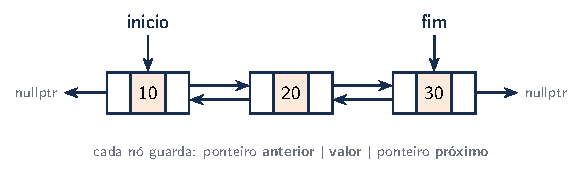
\includegraphics[width=0.95\linewidth,keepaspectratio]{imagens/capitulo-03_dupla.pdf}
\end{center}

Com os dois ponteiros, inserir e remover nas duas pontas custa $O(1)$, e a lista pode ser percorrida nos dois sentidos. O preço é um ponteiro a mais por nó e mais cuidado: cada operação precisa manter \texttt{anterior} e \texttt{proximo} coerentes.

\begin{codigo}
\begin{Verbatim}[breaklines=true, breaksymbolleft={}, fontsize=\footnotesize]
struct NoDuplo {
    int valor;
    NoDuplo *anterior;
    NoDuplo *proximo;
};

class ListaDupla {
private:
    NoDuplo *inicio;
    NoDuplo *fim;
    int tamanho;

public:
    ListaDupla() : inicio(nullptr), fim(nullptr), tamanho(0) {}

    ~ListaDupla() {
        while (!vazia()) {
            removerInicio();
        }
    }

    ListaDupla(const ListaDupla &) = delete;
    ListaDupla &operator=(const ListaDupla &) = delete;

    bool vazia() const { return tamanho == 0; }

    void inserirInicio(int valor) {
        NoDuplo *novo = new NoDuplo{valor, nullptr, inicio};
        if (inicio == nullptr) {
            fim = novo;
        } else {
            inicio->anterior = novo;
        }
        inicio = novo;
        tamanho++;
    }

    void inserirFim(int valor) {
        NoDuplo *novo = new NoDuplo{valor, fim, nullptr};
        if (fim == nullptr) {
            inicio = novo;
        } else {
            fim->proximo = novo;
        }
        fim = novo;
        tamanho++;
    }

    // as duas remoções são O(1): não é preciso procurar o vizinho
    bool removerInicio() {
        if (vazia()) return false;
        NoDuplo *velho = inicio;
        inicio = inicio->proximo;
        if (inicio == nullptr) {
            fim = nullptr;           // a lista ficou vazia
        } else {
            inicio->anterior = nullptr;
        }
        delete velho;
        tamanho--;
        return true;
    }

    bool removerFim() {
        if (vazia()) return false;
        NoDuplo *velho = fim;
        fim = fim->anterior;         // o penúltimo, sem precisar procurar
        if (fim == nullptr) {
            inicio = nullptr;
        } else {
            fim->proximo = nullptr;
        }
        delete velho;
        tamanho--;
        return true;
    }

    void imprimir() const {
        for (NoDuplo *a = inicio; a != nullptr; a = a->proximo) cout << a->valor << " ";
        cout << endl;
    }

    void imprimirInvertido() const {
        for (NoDuplo *a = fim; a != nullptr; a = a->anterior) cout << a->valor << " ";
        cout << endl;
    }
};

int main() {
    ListaDupla lista;
    lista.inserirFim(20);
    lista.inserirFim(30);
    lista.inserirInicio(10);
    lista.imprimir();            // 10 20 30
    lista.imprimirInvertido();   // 30 20 10
    lista.removerFim();
    lista.removerInicio();
    lista.imprimir();            // 20
}
\end{Verbatim}
\end{codigo}

\subsection{3.9 Lista circular}

Em uma \textbf{lista circular}, o último nó não aponta para \texttt{nullptr}: aponta de volta para o primeiro. A lista vira um anel, sem começo nem fim naturais.

\begin{center}
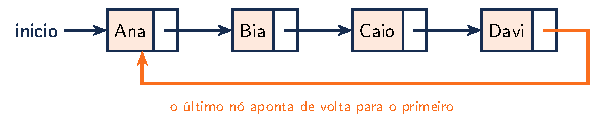
\includegraphics[width=0.95\linewidth,keepaspectratio]{imagens/capitulo-03_circular.pdf}
\end{center}

Ela é útil sempre que os elementos são atendidos em rodízio, voltando ao primeiro depois do último: turnos de um jogo, a fila de processos que dividem o processador, as músicas de uma playlist em repetição.

Um detalhe elegante: basta guardar um ponteiro para o \textbf{último} nó. O primeiro é sempre \texttt{ultimo->proximo}, então as duas pontas ficam acessíveis em $O(1)$ com um único ponteiro.

\begin{codigo}
\begin{Verbatim}[breaklines=true, breaksymbolleft={}, fontsize=\footnotesize]
struct Jogador {
    string nome;
    Jogador *proximo;
};

class Rodizio {
private:
    Jogador *ultimo = nullptr;   // ultimo->proximo é o primeiro

public:
    ~Rodizio() {
        if (ultimo == nullptr) return;
        Jogador *atual = ultimo->proximo;
        ultimo->proximo = nullptr;          // abre o anel para poder parar
        while (atual != nullptr) {
            Jogador *seguinte = atual->proximo;
            delete atual;
            atual = seguinte;
        }
    }

    Rodizio() = default;
    Rodizio(const Rodizio &) = delete;
    Rodizio &operator=(const Rodizio &) = delete;

    void adicionar(const string &nome) {
        Jogador *novo = new Jogador{nome, nullptr};
        if (ultimo == nullptr) {
            novo->proximo = novo;           // um só jogador: aponta para si mesmo
        } else {
            novo->proximo = ultimo->proximo; // o novo aponta para o primeiro
            ultimo->proximo = novo;          // o antigo último aponta para o novo
        }
        ultimo = novo;                       // o novo passa a ser o último
    }

    void jogar(int turnos) const {
        if (ultimo == nullptr) return;
        Jogador *vez = ultimo->proximo;      // começa pelo primeiro
        for (int t = 1; t <= turnos; t++) {
            cout << "Turno " << t << ": " << vez->nome << endl;
            vez = vez->proximo;              // depois do último, volta ao primeiro
        }
    }
};

int main() {
    Rodizio jogo;
    jogo.adicionar("Ana");
    jogo.adicionar("Bia");
    jogo.adicionar("Caio");
    jogo.jogar(5);   // Ana, Bia, Caio, Ana, Bia
}
\end{Verbatim}
\end{codigo}

Cuidado com a parada: em uma lista circular, percorrer até encontrar \texttt{nullptr} gera um laço infinito. Por isso o percurso para por contagem (como em \texttt{jogar}) ou ao voltar ao nó de partida, e o destrutor ``abre'' o anel antes de liberar os nós.

\subsection{3.10 Vetor ou lista encadeada?}

Nenhuma das duas estruturas é melhor em tudo. A escolha depende de quais operações o seu problema faz com mais frequência:

\begin{center}
\begin{tabular}{@{}p{0.34\linewidth}p{0.16\linewidth}p{0.18\linewidth}p{0.16\linewidth}@{}}
\toprule
\rowcolor{headergray}
\tblheader{Operação} & \tblheader{Vetor} & \tblheader{Lista simples} & \tblheader{Lista dupla} \\
\midrule
Acessar a posição $i$ & $O(1)$ & $O(n)$ & $O(n)$ \\
\rowcolor{rowgray} Inserir no início & $O(n)$ & $O(1)$ & $O(1)$ \\
Inserir no fim & $O(1)$* & $O(1)$ & $O(1)$ \\
\rowcolor{rowgray} Remover do início & $O(n)$ & $O(1)$ & $O(1)$ \\
Remover do fim & $O(1)$ & $O(n)$ & $O(1)$ \\
\rowcolor{rowgray} Buscar um valor & $O(n)$ & $O(n)$ & $O(n)$ \\
Memória extra por elemento & nenhuma & 1 ponteiro & 2 ponteiros \\
\bottomrule
\end{tabular}
\end{center}

{\footnotesize * No vetor dinâmico, quase sempre $O(1)$; de vez em quando, quando enche, a cópia para um espaço maior custa $O(n)$. Na média, continua $O(1)$: dizemos que é $O(1)$ \textbf{amortizado}.}

Em resumo: prefira o \textbf{vetor} quando o acesso por posição for frequente e as inserções acontecerem no fim; prefira a \textbf{lista} quando houver muitas inserções e remoções nas pontas ou no meio de uma sequência que você já está percorrendo. Na prática, vetores também se beneficiam de estarem contínuos na memória, o que o processador aproveita muito bem; por isso, para listas pequenas, o vetor costuma ser mais rápido mesmo quando a tabela sugere o contrário.

\begin{destaque}{Comparando com Python}
A \texttt{list} do Python é um vetor dinâmico, não uma lista encadeada: acessar \texttt{lista[i]} é $O(1)$, mas \texttt{lista.insert(0, x)} é $O(n)$. Quando você precisa inserir e remover nas duas pontas, a escolha certa é o \texttt{deque}, do módulo \texttt{collections}, implementado com blocos encadeados. E, se quiser, dá para escrever uma lista encadeada em Python com a mesma ideia de nós:

\begin{codigo}
\begin{Verbatim}[breaklines=true, breaksymbolleft={}, fontsize=\footnotesize]
from collections import deque

class No:
    def __init__(self, valor, proximo=None):
        self.valor = valor
        self.proximo = proximo     # referência para o próximo nó (ou None)

inicio = No(10, No(20, No(30)))   # 10 -> 20 -> 30
atual = inicio
while atual is not None:
    print(atual.valor, end=" ")
    atual = atual.proximo
print()

pedidos = deque([20, 30])
pedidos.appendleft(10)           # O(1), como inserirInicio
pedidos.append(40)               # O(1), como inserirFim
print(pedidos.popleft())         # 10, O(1)
\end{Verbatim}
\end{codigo}

Em Python não há \texttt{delete}: quando nenhum nó aponta mais para um objeto, a coleta de lixo o remove.
\end{destaque}

A biblioteca padrão do C++ também oferece listas prontas: \texttt{std::forward\_list} (simplesmente encadeada) e \texttt{std::list} (duplamente encadeada). Agora que você sabe como funcionam por dentro, use-as nos seus projetos.

\subsection{Erros Comuns}

\begin{itemize}
  \item \textbf{Perder o resto da lista.} Ao inserir no início, atualizar \texttt{inicio} antes de ligar o novo nó ao antigo primeiro deixa todos os outros nós inacessíveis.
  \item \textbf{Esquecer a lista vazia.} Toda operação precisa funcionar quando \texttt{inicio} é \texttt{nullptr}. Acessar \texttt{inicio->valor} em uma lista vazia derruba o programa.
  \item \textbf{Não atualizar o ponteiro \texttt{fim}.} Ao remover o último nó, \texttt{fim} precisa passar a apontar para o anterior (ou para \texttt{nullptr}, se a lista ficou vazia).
  \item \textbf{Usar o nó depois do \texttt{delete}.} No destrutor, guarde o \texttt{proximo} em uma variável \textit{antes} de liberar o nó atual.
  \item \textbf{Esquecer o destrutor.} Sem ele, todos os nós ficam presos na memória quando a lista deixa de existir.
  \item \textbf{Copiar uma lista sem tratar a cópia.} A cópia automática divide os mesmos nós entre duas listas e causa \texttt{delete} duplo. Proíba a cópia ou implemente-a nó por nó.
  \item \textbf{Esquecer um dos ponteiros na lista dupla.} Cada inserção e remoção precisa atualizar \texttt{anterior} e \texttt{proximo} dos vizinhos.
  \item \textbf{Laço infinito na lista circular.} Na lista circular, nenhum nó aponta para \texttt{nullptr}: o percurso precisa parar por contagem ou ao voltar ao início.
\end{itemize}
